\documentclass[11pt,notes=hide,aspectratio=169,mathserif]{beamer}

% PACKAGES
\usepackage{graphics}
\usepackage{graphicx}  % \resizebox
\usepackage{url}
%\usepackage{natbib}
\usepackage{bibentry}
\usepackage{verbatim}
\usepackage{booktabs}
\usepackage{etoolbox}
\usepackage{datetime}
\usepackage{bm}
\usepackage{subcaption}
\usepackage{amsfonts}
\usepackage{amsmath}
\usepackage{amsthm}

% CUSTOM DEFINITIONS
\def\newblock{} % Get beamer to cooperate with BibTeX
\linespread{1.2}

% IDENTIFYING INFORMATION
\title[class]{ECON 344: Economics of Crime \\ TA Session 2}
\author[vaidehi's class ]{Vaidehi Parameswaran (Northwestern Economics)}
\date{\monthname[\the\month] \the\year}

% THEME OPTIONS
\definecolor{mycolor}{RGB}{0,105,105}
\setbeamercolor{normal text}{fg=black,bg=white}
\setbeamercolor{title}{fg=mycolor}
\setbeamercolor{frametitle}{fg=mycolor,bg=white}
\setbeamercolor{section in toc}{fg=mycolor}
\setbeamerfont{frametitle}{series=\bfseries}
\setbeamerfont{title}{series=\bfseries}
\beamertemplatenavigationsymbolsempty
\setbeamertemplate{footline}{%
  \hfill
  \usebeamerfont{page number in head/foot}
  \usebeamercolor[fg]{page number in head/foot}
  \insertframenumber\hspace{0.6cm}\vspace{0.25cm}
}
\setbeamercolor{page number in head/foot}{fg=gray}
\setbeamertemplate{itemize item}{\small\raisebox{1pt}{\textcolor{mycolor}{$\blacktriangleright$}}}
\setbeamertemplate{itemize subitem}{\footnotesize\raisebox{1pt}{\textcolor{mycolor}{$\triangleright$}}}
\setbeamertemplate{itemize subsubitem}{\tiny\raisebox{1pt}{\textcolor{mycolor}{$\triangleright$}}}

% Clickable links
\usepackage{hyperref}
\hypersetup{
  colorlinks=true,
  linkcolor=mycolor,
  urlcolor=mycolor,
  citecolor=mycolor
}

% BACKUP SLIDE NUMBERING
\usepackage{appendixnumberbeamer}

% Show a bulleted mini-contents slide at each section
% Bulleted ToC using your triangle icons + color
\setbeamertemplate{section in toc}{%
  \leavevmode\llap{\textcolor{mycolor}{$\blacktriangleright$}\hspace{0.6ex}}%
  \inserttocsection\par}
\setbeamertemplate{subsection in toc}{%
  \leavevmode\llap{\textcolor{mycolor}{$\triangleright$}\hspace{1.1ex}}%
  \inserttocsubsection\par}

\AtBeginSection[]{
\begin{frame}{Today}
\tableofcontents[currentsection]
\ifnum\value{section}=3
\vspace{1em}
\href{https://www.journals.uchicago.edu/doi/full/10.1086/716561}
{\textcolor{mycolor}{\underline{Rose \& Shem-Tov (2021): How Does Incarceration Affect Reoffending?}}}
\fi
\ifnum\value{section}=4
\vspace{1em}
\href{https://doi.org/10.1162/REST_a_00484}
{\textcolor{mycolor}{\underline{Freedman \& Owens (2016): Your Friends and Neighbors}}}
\fi
\end{frame}
}

\begin{document}

%---------------------------------------------------------------------
\begin{frame}[plain]
\titlepage
\end{frame}
%---------------------------------------------------------------------

\section{Introductions}
%---------------------------------------------------------------------
\begin{frame}{Introductions}
\begin{itemize}
  \item Me: a fourth-year grad student in the econ department
  \begin{itemize}
    \item Interested in applied microeconomics, labour, gender
    \item Email: \textcolor{blue}{vaidehiparameswaran2029@u.northwestern.edu}
    \item Office hours: Tuesdays, 9--11am in KGH 3411
  \end{itemize}
\end{itemize}
\end{frame}
%---------------------------------------------------------------------

%---------------------------------------------------------------------

\section{Becker Model of Crime}

%---------------------------------------------------------------------
\begin{frame}{The Becker Model of Crime}
\begin{itemize}
\item Becker (1968): treat criminal activity as a \textbf{rational choice under uncertainty}
\pause \item A potential offender compares the expected payoff from committing a crime to the payoff from not committing it
\pause \item Crime depends on:
\begin{itemize}
    \item the benefits from committing crime
    \item the expected costs of crime, including the probability and severity of punishment
    \item opportunities outside of crime
\end{itemize}
\end{itemize}
\end{frame}
%---------------------------------------------------------------------

%---------------------------------------------------------------------
\begin{frame}{The Individual's Decision}
\begin{itemize}
\item Suppose an individual receives:
\begin{itemize}
    \item $U_{nc}$ from not committing crime
    \item $U_{c1}$ from committing crime and being caught
    \item $U_{c2}$ from committing crime and not being caught
\end{itemize}
\pause \item Let $p$ be the probability of being caught
\pause \item Expected utility from crime is:
\pause
\[
pU_{c1}+(1-p)U_{c2}
\]
\pause \item The individual commits crime if:
\pause
\[
\underbrace{pU_{c1}+(1-p)U_{c2}}_{\text{expected utility from crime}}
>
\underbrace{U_{nc}}_{\text{utility from not committing crime}}
\]
\end{itemize}
\end{frame}
%---------------------------------------------------------------------

%---------------------------------------------------------------------
\begin{frame}{What Changes the Incentive to Commit Crime?}
\begin{itemize}
\item Becker writes expected utility from crime as:
\[
EU=pU(Y-f)+(1-p)U(Y)
\]
where $Y$ is the payoff from crime and $f$ is the punishment if caught
\pause \item Crime becomes less attractive when:
\begin{itemize}
    \pause \item probability of apprehension $p$ increases
    \pause \item severity of punishment $f$ increases
\end{itemize}
\pause \item Crime also becomes less attractive when \textbf{outside opportunities improve}
\begin{itemize}
    \item e.g.\ higher wages or better employment opportunities increase the opportunity cost of crime
\end{itemize}
\end{itemize}
\end{frame}
%---------------------------------------------------------------------

%---------------------------------------------------------------------
\begin{frame}{Optimal Enforcement}
\begin{itemize}
\item Becker also asks: how should society choose enforcement and punishment?
\pause \item The planner trades off:
\begin{itemize}
    \item harm caused by crime
    \item gains to offenders
    \item cost of policing and apprehension
    \item social cost of punishment
\end{itemize}
\pause \item For a risk-neutral offender:
\[
EU = G - pf
\]
so deterrence depends on the \textbf{expected punishment} $pf$
\pause \item Holding $pf$ fixed, society could reduce costly enforcement $p$ and increase punishment $f$
\end{itemize}
\end{frame}
%---------------------------------------------------------------------


\section{Incarceration and Reoffending}


%---------------------------------------------------------------------
\begin{frame}{Incarceration}
\begin{itemize}
\item Incarceration rate in the US has more than tripled since the 1980s
\end{itemize}
\begin{figure}
\centering
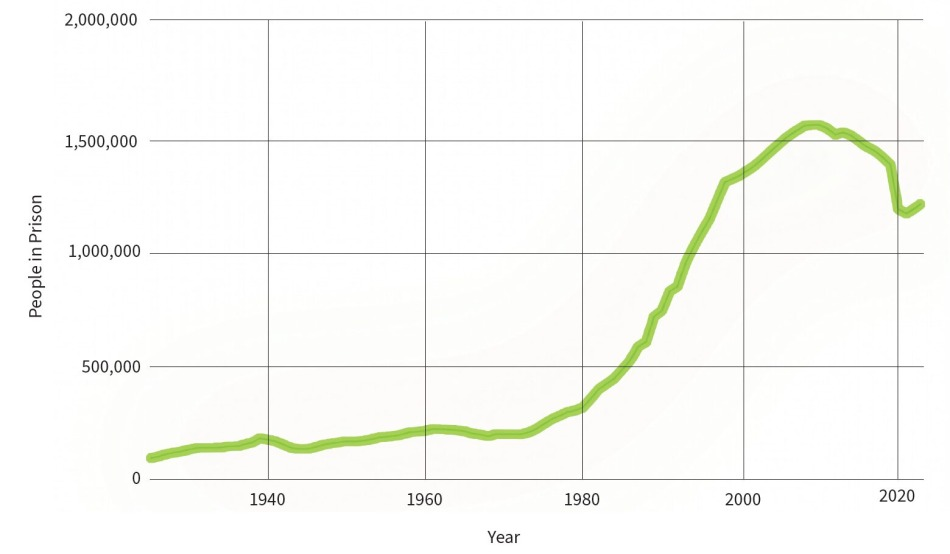
\includegraphics[width=0.5\textwidth]{inputs/incarceration_rate2.png}
\end{figure}
Naturally, we would want to know whether this increase in incarceration has reduced crime
\end{frame}
%---------------------------------------------------------------------


%---------------------------------------------------------------------
\begin{frame}{Crime rates have been declining over this time period}
\begin{figure}
\centering
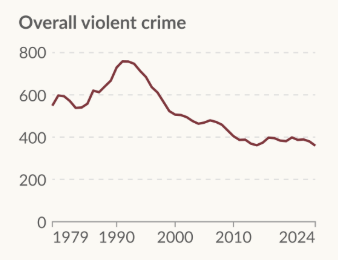
\includegraphics[width=0.5\textwidth]{inputs/crime.png}
\end{figure}
Can we conclude from these data that incarceration has reduced crime?
\end{frame}
%---------------------------------------------------------------------



%---------------------------------------------------------------------
\begin{frame}{Research Question}
\begin{itemize}
\item Incarceration could affect future crime in several ways
\pause \item It may reduce crime through:
\begin{itemize}
\pause \item \textbf{incapacitation}: people cannot commit crimes outside prison while incarcerated
\pause \item \textbf{deterrence}: punishment discourages future crime
\pause \item \textbf{rehabilitation}: prison changes behavior or provides services
\end{itemize}
\pause \item It may also increase crime
\begin{itemize}
\pause \item prison may disrupt employment and family ties
\pause \item prison may expose people to criminal networks
\end{itemize}
\pause \item Open question: How does incarceration affect reoffending?
\pause \item And more specifically: how does the effect vary with sentence length?
\end{itemize}
\end{frame}
%---------------------------------------------------------------------

%---------------------------------------------------------------------
\begin{frame}{Why Is This Hard to Estimate?}
\begin{itemize}
\item Suppose we compare people sentenced to prison with people sentenced to probation or fines
\item \textbf{Question:} Would this identify the causal effect of incarceration?
\pause \item No: incarceration is endogenous
\begin{itemize}
\pause \item more serious offenders are more likely to be sent to prison
\pause  \item people with longer criminal histories receive harsher sentences
\pause  \item judges may observe risk factors researchers do not observe
\end{itemize}
\pause \item Naive comparison:
\[
\text{Reoffend}_i=\alpha+\beta \text{Prison}_i+\epsilon_i
\]
\pause \item $\beta$ combines the effect of prison with selection into prison
\pause \item $\Rightarrow$ Need variation in incarceration that is not driven by underlying reoffending risk
\end{itemize}
\end{frame}
%---------------------------------------------------------------------


%---------------------------------------------------------------------
\begin{frame}{Setting: North Carolina Sentencing Guidelines}
\begin{itemize}
\item North Carolina uses structured sentencing guidelines
\pause \item Sentences depend on two main inputs:
\begin{enumerate}
\item offense severity
\item prior record points
\end{enumerate}
\pause \item Prior record points summarize criminal history
\begin{itemize}
\item one point for misdemeanor offenses and two to 10 points for felony offenses
\item crossing certain thresholds moves a defendant into a harsher sentencing cell
\end{itemize}
\pause \item Key idea:
\[
\text{similar defendants on either side of a cutoff face different sentence recommendations}
\]
\pause \item \textbf{Question:} Why might this be useful for causal inference?
\end{itemize}
\end{frame}
%---------------------------------------------------------------------

%---------------------------------------------------------------------
\begin{frame}{Identification Strategy}
\begin{itemize}
\item Running variable:
\[
\text{prior record points}
\]
\pause \item Outcomes:
\begin{itemize}
\item new arrests
\item new felony offenses
\item reincarceration within 3, 5, or 8 years
\end{itemize}
\pause \item Basic comparison:
\text{defendants just below a sentencing threshold vs. just above}
\pause \item $\Rightarrow$ A regression-discontinuity design
\end{itemize}
\end{frame}
%---------------------------------------------------------------------

%---------------------------------------------------------------------
\begin{frame}{What Must Be True for the Design to Work?}
\begin{itemize}
\item \textbf{Relevance:} crossing the threshold must change incarceration (first stage)
\pause \item \textbf{Continuity:} defendants just below and just above the threshold must be otherwise comparable
\pause \item \textbf{No manipulation:} defendants, prosecutors, or judges should not precisely sort cases around the cutoff
\pause \item \textbf{Exclusion restriction:} the threshold should affect reoffending only through the sentence
% \pause \item \textbf{Question:} Which assumption worries you most?
% \pause \item Main concern: charges and plea bargaining may affect where someone lands in the sentencing grid
\end{itemize}
\end{frame}
%---------------------------------------------------------------------

%---------------------------------------------------------------------
\begin{frame}{First Stage}
\begin{itemize}
\item First stage: crossing guideline thresholds creates large jumps in incarceration
\begin{itemize}
\item example: for some offenses, the probability of incarceration jumps sharply at the cutoff
\end{itemize}
\end{itemize}
\begin{figure}
\centering
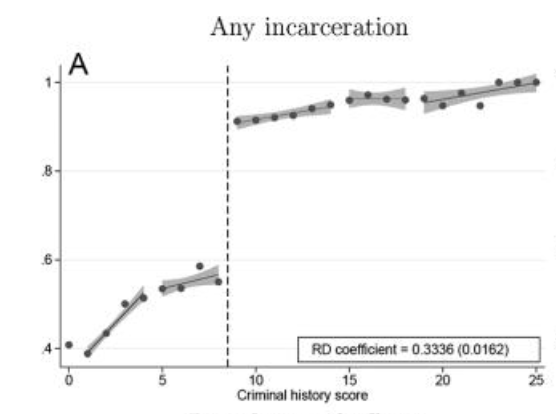
\includegraphics[width=0.5\textwidth]{inputs/first_stage.png}
\end{figure}
\end{frame}
%---------------------------------------------------------------------

%---------------------------------------------------------------------
\begin{frame}{Continuity and Balance Checks}
\begin{itemize}
\item Validity checks ask whether defendants also change discontinuously at the threshold
\pause \item These characteristics evolve smoothly across the thresholds
\end{itemize}
\only<3>{
\begin{center}
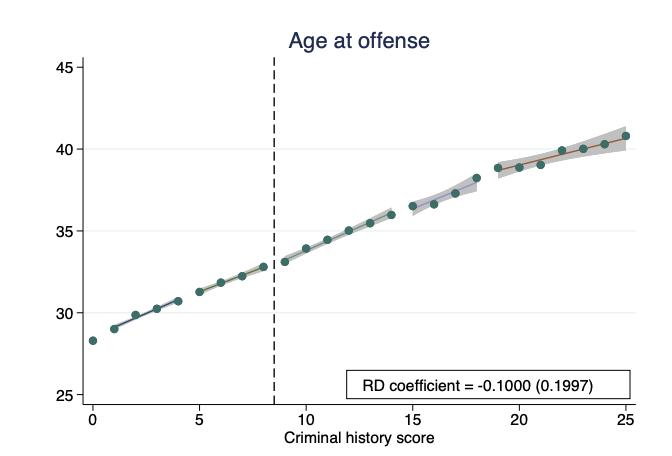
\includegraphics[width=0.5\textwidth]{inputs/age.png}
\end{center}
}
\only<4>{
\begin{center}
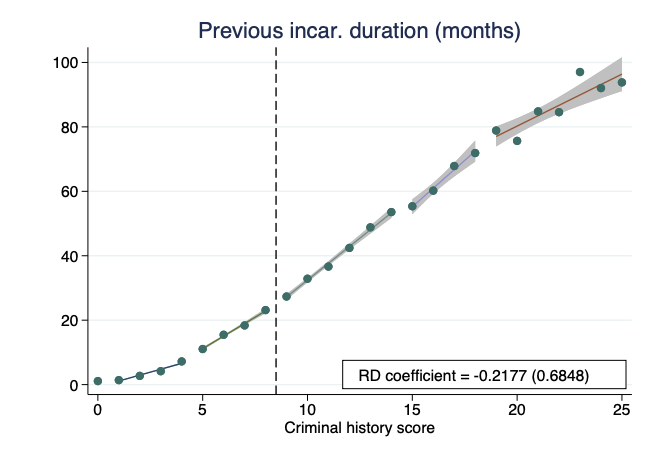
\includegraphics[width=0.5\textwidth]{inputs/prev_incar.png}
\end{center}
}
\end{frame}
%---------------------------------------------------------------------

%---------------------------------------------------------------------
\begin{frame}{Main Result: Does Incarceration Reduce Reoffending?}
\begin{itemize}
\item \textbf{Yes.} The RD/IV estimates suggest incarceration reduces future offending
\begin{figure}
\centering
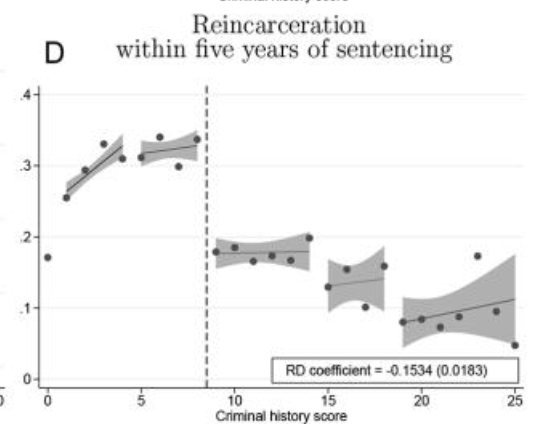
\includegraphics[width=0.5\textwidth]{inputs/reincar.png}
\end{figure}
\end{itemize}
\end{frame}
%---------------------------------------------------------------------


%---------------------------------------------------------------------
\begin{frame}{By How Much?}
\begin{figure}
\centering
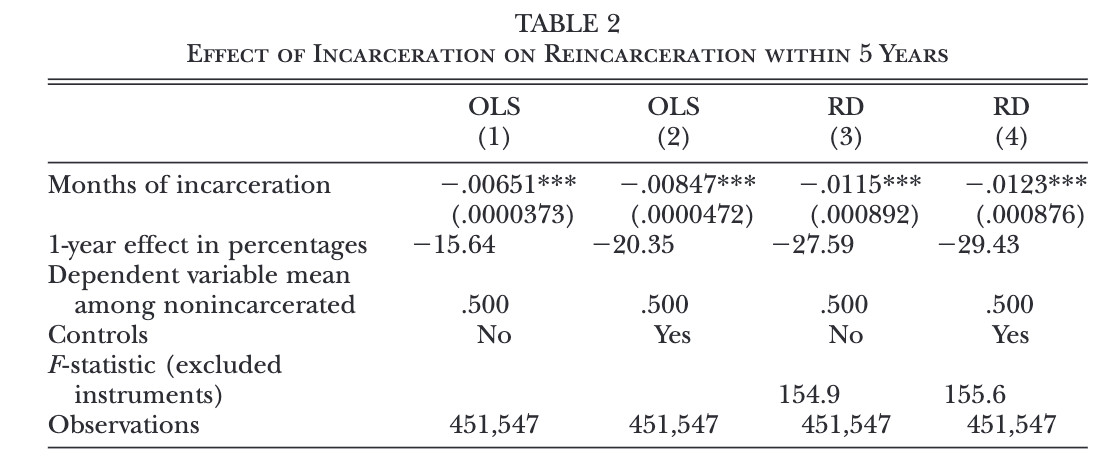
\includegraphics[width=0.8\textwidth]{inputs/rdd_table.png}
\end{figure}
\begin{itemize}
\pause \item One year of incarceration reduces reincarceration within 5 years by about \textbf{13.8 p.p.}
\begin{itemize}
\item roughly a \textbf{28--29\%} decline relative to the nonincarcerated mean
\end{itemize}
\pause \item Why is OLS less negative than the RDD estimate?
\pause \begin{itemize}
  \item Positive selection $\rightarrow$ upward bias towards zero
\end{itemize}
\end{itemize}
\end{frame}
%---------------------------------------------------------------------

%---------------------------------------------------------------------
\begin{frame}{By Offense Type}
\begin{figure}
\centering
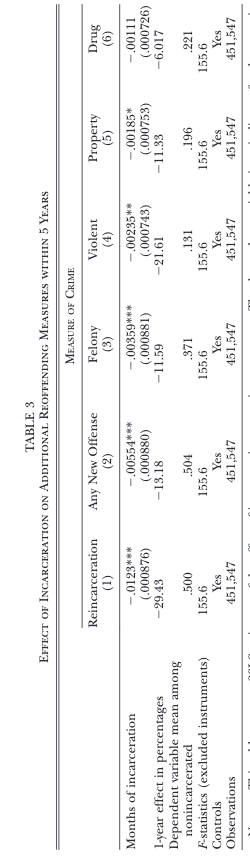
\includegraphics[width=0.3\textwidth,angle=270]{inputs/offense_types.png}
\end{figure}
Reduces the probability of any new offense, including felony, violent, and property offenses
\end{frame}
%---------------------------------------------------------------------

%---------------------------------------------------------------------
\begin{frame}{Why Study the Dose-Response Function?}
\begin{itemize}
\item The main result tells us the effect of more incarceration on average
\pause \item But policymakers need to know:
\begin{itemize}
\item Is the first year of prison more effective than later years?
\item Do longer sentences keep reducing crime at the same rate?
\item Are judges giving longer sentences to people for whom prison has larger effects?
\end{itemize}
\pause \item \textbf{Question:} Why might the first year matter more than the third or fourth year?
\pause \item Possible reason:
\begin{itemize}
\item the first year moves someone from probation to prison
\item later years extend incarceration for people already incapacitated
\end{itemize}
\end{itemize}
\end{frame}
%---------------------------------------------------------------------

%---------------------------------------------------------------------
\begin{frame}{Dose Response and Selection}
\begin{itemize}
\item The paper finds that effects are \textbf{nonlinear}
\pause \item The first year of incarceration has the largest crime-reducing effect
\pause \item Additional years still reduce reoffending, but by less
\begin{itemize}
\item People receiving longer prison sentences are higher risk
\item But they also appear to have larger reductions in reoffending from incarceration
\end{itemize}
\end{itemize}
\end{frame}
%---------------------------------------------------------------------

%---------------------------------------------------------------------
\begin{frame}{Discussion and Takeaways}
\begin{itemize}
\item \textbf{Main result:} incarceration reduces subsequent reoffending in this setting
\pause \item What should we worry about for identification?
\begin{itemize}
\item Continuity/manipulation: could defendants, prosecutors, or judges sort cases around the sentencing thresholds?
\item Exclusion restriction: could crossing a threshold change outcomes through something other than incarceration?
\end{itemize}
\pause \item How does this speak to Becker's model of crime?
\begin{itemize}
\pause \item Incarceration is a more severe punishment, so it relates to Becker's $f$
\item But incarceration also mechanically prevents offending while someone is in prison (\textbf{incapacitation})
\item The estimates therefore do not isolate the ex ante deterrence effect emphasized by Becker
\end{itemize}
\pause \item $\Rightarrow$ The paper shows that incarceration can reduce reoffending, but understanding \textit{why} matters for interpreting the policy implications
\end{itemize}
\end{frame}
%---------------------------------------------------------------------



%---------------------------------------------------------------------
\section{Economic Development and Criminal Activity}
%---------------------------------------------------------------------

%---------------------------------------------------------------------
\begin{frame}{From Becker to Neighborhood Spillovers}
\begin{itemize}
\item Becker: higher opportunity costs should reduce crime
\[
\uparrow U_{nc} \quad \Rightarrow \quad \downarrow \text{crime}
\]
\item So should better labor market opportunities reduce crime?
\pause \item But if only some people benefit, could the others be incentivized to commit more crime?
\pause \item Economic development may affect people differently within the same neighborhood
\pause \item Freedman \& Owens study this using a localized economic shock in San Antonio
\end{itemize}
\end{frame}
%---------------------------------------------------------------------

%---------------------------------------------------------------------
\begin{frame}{Research Question}
\begin{itemize}
\item Most of the literature asks:
\[
\text{Do better legal labor-market opportunities reduce crime?}
\]
\pause \item This paper asks a slightly different question:
\[
\text{What happens when some neighbors benefit economically, but others do not?}
\]
\pause \item Two competing forces:
\begin{itemize}
\item \textbf{Legal employment:} beneficiaries have more to lose from crime
\item \textbf{Criminal opportunity:} non-beneficiaries may face richer nearby targets
\end{itemize}
\pause \item \textbf{Question:} Which effect should dominate?
\end{itemize}
\end{frame}
%---------------------------------------------------------------------

%---------------------------------------------------------------------
\begin{frame}{Setting: BRAC in San Antonio}
\begin{itemize}
\item In 2005, the Base Realignment and Closure program expanded military activity in San Antonio
\pause \item This created a large, localized increase in demand for construction labor in 2007-2010
\pause \item Why construction?
\begin{itemize}
\item BRAC required substantial new building and renovation
\item Much of the local economic impact came through construction jobs
\item Eligibility based on background checks and ID verification
\end{itemize}
\pause \item Neighborhoods differed in how exposed they were
\begin{itemize}
\item high construction-worker neighborhoods were more likely to benefit
\item low construction-worker neighborhoods were less exposed
\end{itemize}
\end{itemize}
\end{frame}
%---------------------------------------------------------------------

%---------------------------------------------------------------------
\begin{frame}{Why Is This a Useful Shock?}
\begin{itemize}
\item A naive comparison of richer and poorer neighborhoods is not causal
\pause \item \textbf{Question:} Why not?
\pause \item Neighborhood economic conditions are endogenous
\begin{itemize}
\item crime can affect investment and employment
\item neighborhoods with different labor markets may differ in policing, demographics, or trends
\end{itemize}
\pause \item BRAC creates a sharper source of variation
\begin{itemize}
\item timing: shock begins after the 2005 BRAC announcement
\item geography: stronger in neighborhoods with more construction workers
\end{itemize}
\pause \item $\Rightarrow$ Difference-in-differences across neighborhoods with different exposure to construction demand
\end{itemize}
\end{frame}
%---------------------------------------------------------------------

%---------------------------------------------------------------------
\begin{frame}{Empirical Strategy}
\begin{itemize}
\item Treatment intensity:
\[
\text{share of neighborhood residents working in construction before BRAC}
\]
\pause \item Post period:
\[
\text{after the 2005 BRAC shock}
\]
\pause \item Basic idea:
\[
\text{Crime}_{nt}=\alpha_n+\lambda_t+\beta(\text{ConstructionShare}_n \times \text{Post}_t)+\epsilon_{nt}
\]
\pause \item Compare high- vs.\ low-construction neighborhoods before and after BRAC
\pause \item Outcome: felony criminal behavior by neighborhood residents
\end{itemize}
\end{frame}
%---------------------------------------------------------------------

%---------------------------------------------------------------------
\begin{frame}{What Is the Identifying Assumption?}
\begin{itemize}
\pause \item \textbf{Parallel trends:}
\pause Absent BRAC, high- and low-construction neighborhoods would have 
followed similar crime trends
\pause \item \textbf{Question:} What evidence would make this more believable?
\pause \item Useful checks:
\begin{itemize}
\item similar pre-trends in crime
\item no other simultaneous shock concentrated in construction-worker neighborhoods
\item observable neighborhood characteristics not changing differentially for unrelated reasons
\end{itemize}
\pause \item \textbf{Main concern:} construction-worker neighborhoods may have been on different crime trajectories even without BRAC
\end{itemize}
\end{frame}
%---------------------------------------------------------------------

%---------------------------------------------------------------------
\begin{frame}{Why Individual-Level Data Matter}
\begin{itemize}
\item Aggregate neighborhood crime could rise for many reasons
\pause \item The paper can ask: \textbf{who commits the additional crimes?}
\pause \item This is important because BRAC jobs were not available to everyone
\begin{itemize}
\item federal construction jobs required background checks
\item people with serious criminal records were unlikely to benefit directly
\end{itemize}
\pause \item Prior:
\begin{itemize}
\item potential beneficiaries should commit less crime
\item non-beneficiaries may commit more crime if opportunities to steal increase
\end{itemize}
\end{itemize}
\end{frame}
%---------------------------------------------------------------------

%---------------------------------------------------------------------
\begin{frame}{Comparison of High- and Low-Construction Neighborhoods}
\begin{figure}
\centering
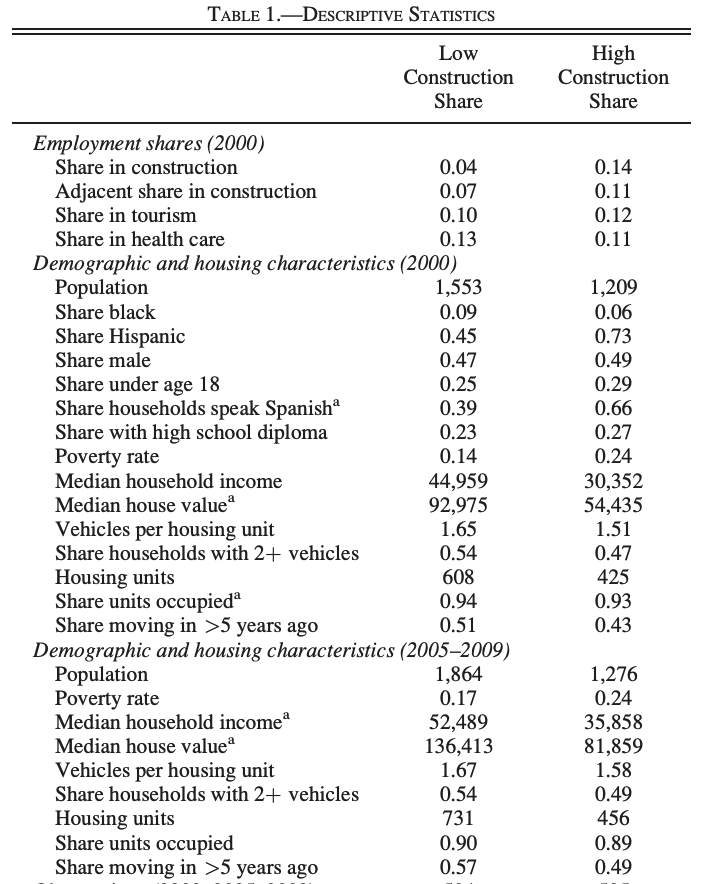
\includegraphics[width=0.5\textwidth]{inputs/desc_table.png}
\end{figure}
\end{frame}
%---------------------------------------------------------------------

%---------------------------------------------------------------------
\begin{frame}{Trends in Crime Before and After BRAC}
\begin{figure}
\centering
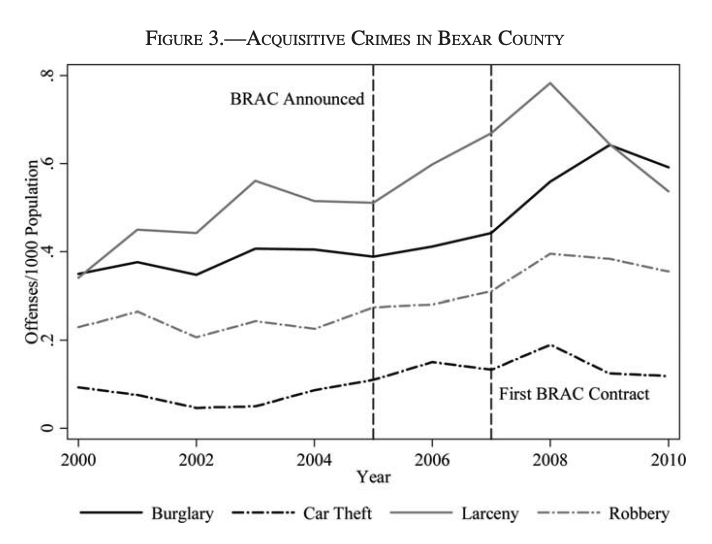
\includegraphics[width=0.7\textwidth]{inputs/trend.png}
\end{figure}
\end{frame}
%---------------------------------------------------------------------

%---------------------------------------------------------------------
\begin{frame}{DiD Result}
\begin{figure}
\centering
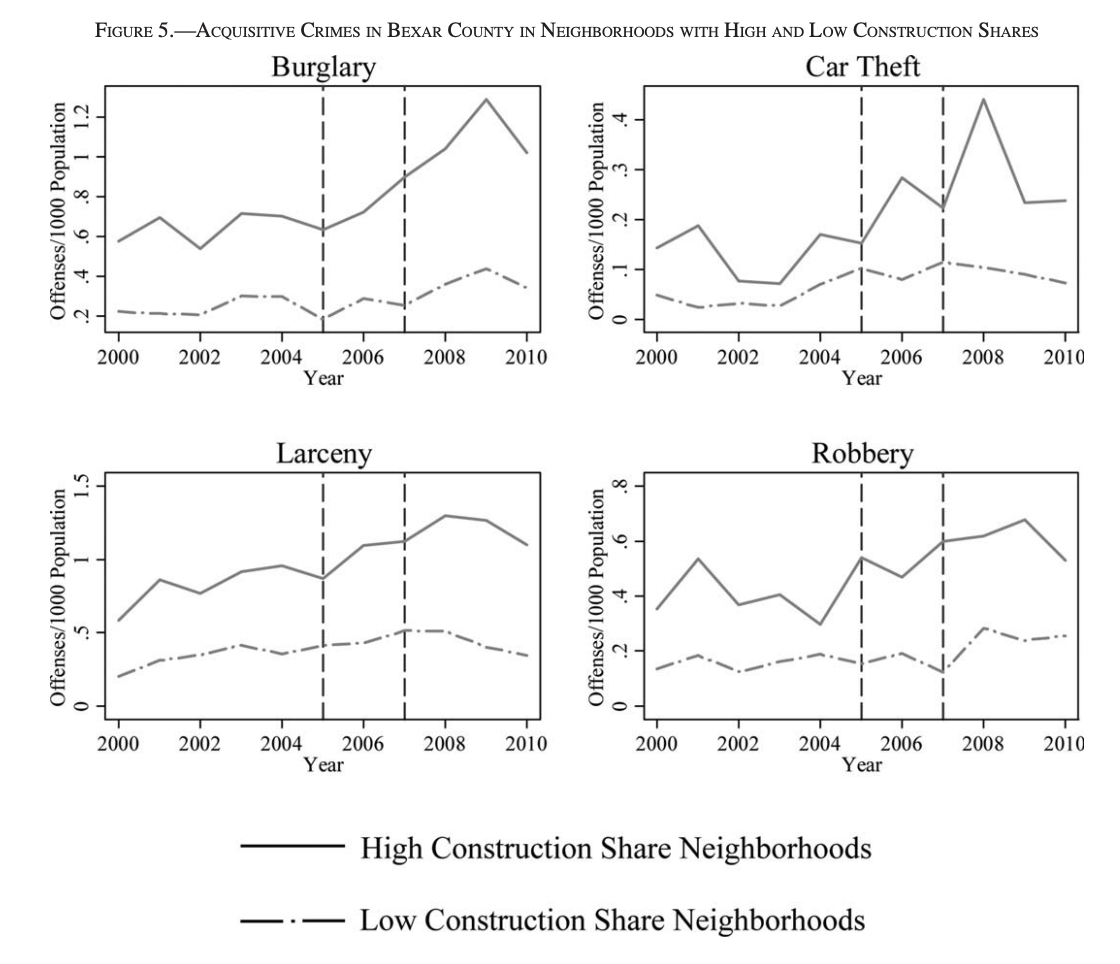
\includegraphics[width=0.65\textwidth]{inputs/did_main.png}
\end{figure}
\end{frame}
%---------------------------------------------------------------------

%---------------------------------------------------------------------
\begin{frame}{DiD Result}
\begin{figure}
\centering
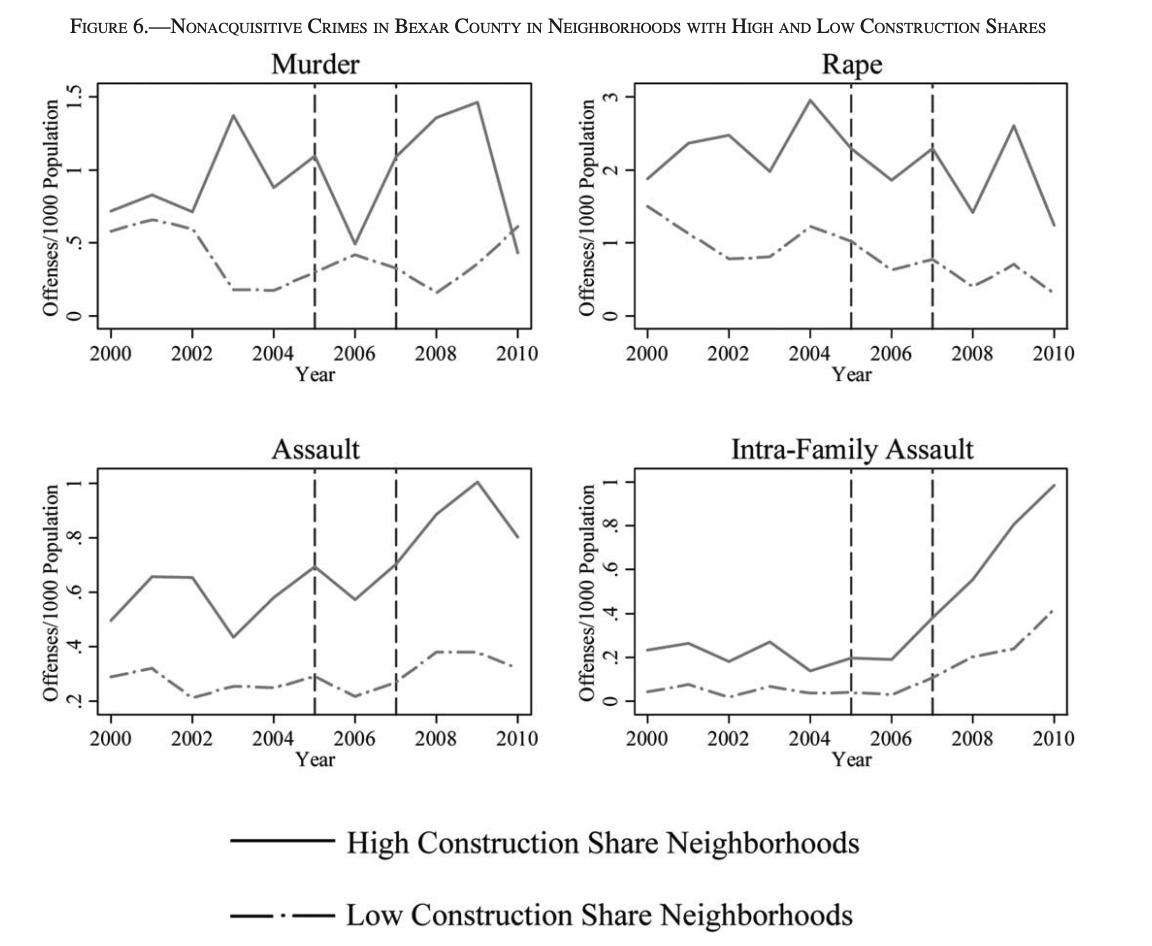
\includegraphics[width=0.65\textwidth]{inputs/did_other.png}
\end{figure}
\end{frame}
%---------------------------------------------------------------------


%---------------------------------------------------------------------
\begin{frame}{DiD Result - Who Commits the Additional Crimes?}
\begin{figure}
\centering
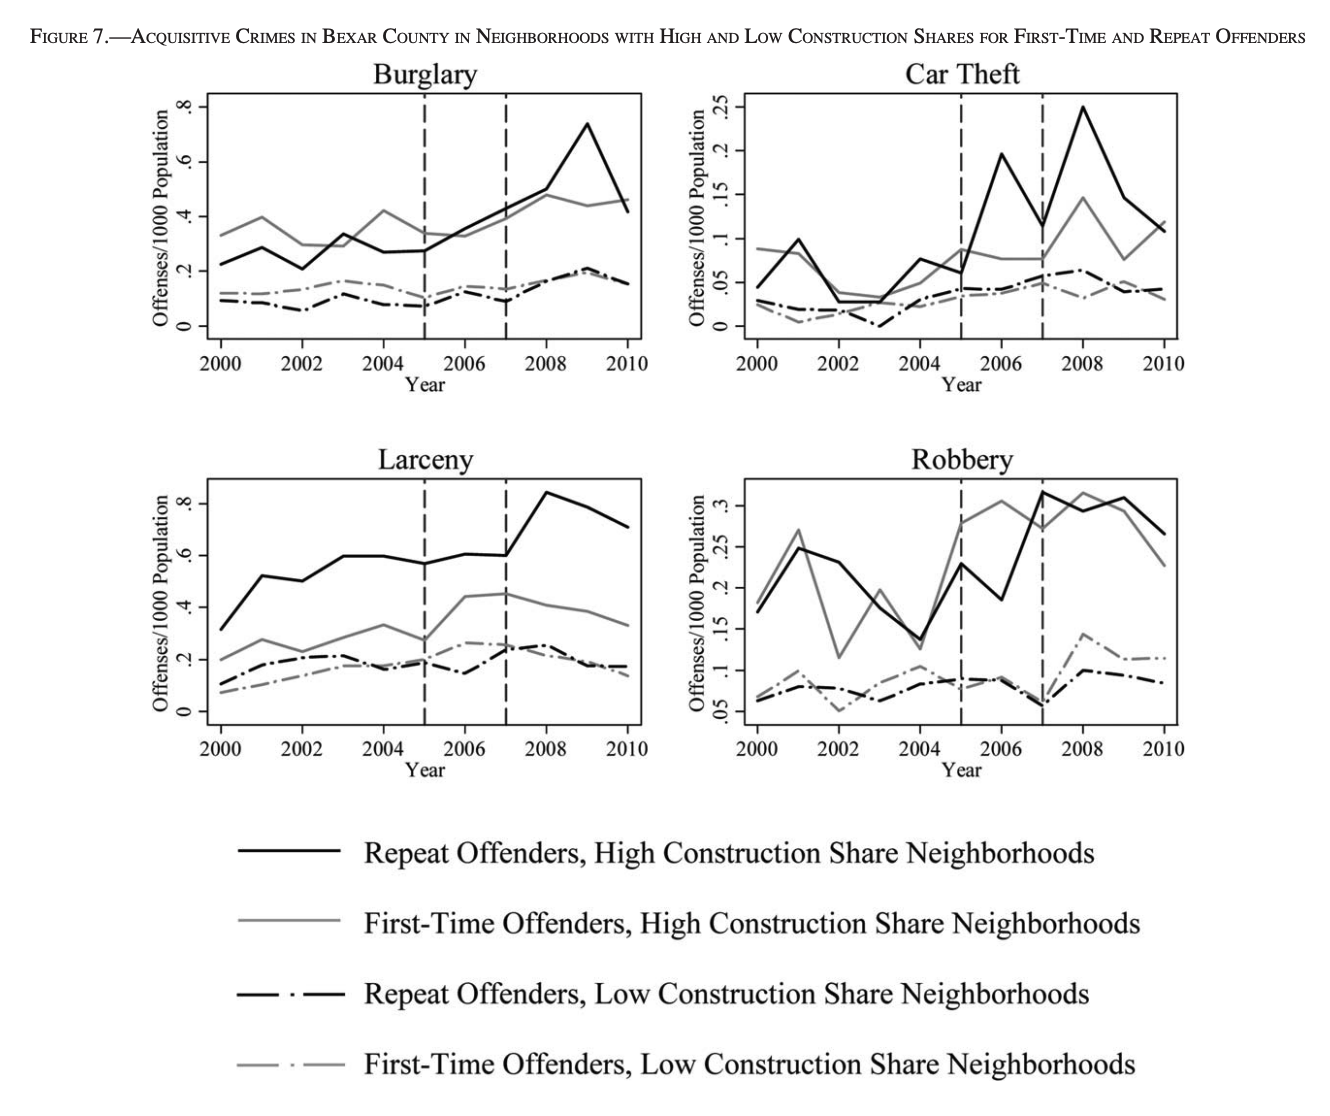
\includegraphics[width=0.65\textwidth]{inputs/who.png}
\end{figure}
\end{frame}
%---------------------------------------------------------------------

%---------------------------------------------------------------------
\begin{frame}{Takeaway}
\begin{itemize}
\item The paper finds that felony behavior increases in more exposed neighborhoods after BRAC
\pause \item The increase is concentrated in \textbf{acquisitive crimes}
\begin{itemize}
\item crimes where material gain is an important motive
\end{itemize}
\pause \item The effect is driven by residents unlikely to benefit directly from BRAC jobs
\begin{itemize}
\item especially people with prior criminal records
\end{itemize}
\pause \item \textbf{Interpretation:} economic development increased criminal opportunities for nearby non-beneficiaries
\end{itemize}
\end{frame}
%---------------------------------------------------------------------

%---------------------------------------------------------------------
\begin{frame}{How Does This Fit In With Becker?}
\begin{itemize}
\item \textbf{Question:} Does the result contradict Becker?
\pause \item Not necessarily
\pause \item For construction workers who benefit:
\[
\uparrow U_{nc} \quad \Rightarrow \quad \downarrow \text{crime}
\]
\pause \item For non-beneficiaries:
\[
\uparrow \text{criminal opportunity} \quad \Rightarrow \quad \uparrow \text{crime}
\]
\pause \item $\Rightarrow$ Economic development changes both:
\begin{itemize}
\item the legal return to work
\item the potential payoff from crime
\end{itemize}
\end{itemize}
\end{frame}
%---------------------------------------------------------------------

%---------------------------------------------------------------------
\begin{frame}{Discussion: Threats to Identification}
\begin{itemize}
\item \textbf{Parallel trends}
\begin{itemize}
\item would high-construction neighborhoods have had different crime trends anyway?
\end{itemize}
\pause \item \textbf{Other local changes}
\begin{itemize}
\item did BRAC also change policing, commuting, population, or neighborhood composition?
\end{itemize}
\pause \item \textbf{Measurement}
\begin{itemize}
\item measured crime depends on arrests/charges, not all criminal activity
\item changes in enforcement could look like changes in crime
\end{itemize}
\pause \item \textbf{Interpretation}
\begin{itemize}
\item increased crime does not imply BRAC was welfare-reducing
\item the paper studies one unintended consequence of localized growth
\end{itemize}
\end{itemize}
\end{frame}
%---------------------------------------------------------------------

%---------------------------------------------------------------------
\begin{frame}{What Does This Paper Teach Us?}
\begin{itemize}
\item Economic development can have heterogeneous effects within a neighborhood
\pause \item Better legal opportunities may reduce crime for direct beneficiaries
\pause \item But growth can also increase criminal opportunities for nearby non-beneficiaries
\pause \item This complicates a simple ``jobs reduce crime'' story
\pause \item \textbf{Broader lesson:} crime depends not only on individual labor-market opportunities, but also on the local distribution of gains from economic growth
\end{itemize}
\end{frame}
%---------------------------------------------------------------------


%---------------------------------------------------------------------
\begin{frame}
\begin{center}{\LARGE See you next time!}\end{center}
\end{frame}
%---------------------------------------------------------------------


% % \beginbackup
% % \appendix
% % \input{sections/appendix.tex}
% % \bibliographystyle{../bib/aeanobold}
% % \nobibliography{../bib/bib.bib}
% % \backupend

\end{document}
